%!TEX root=../document.tex

\section{Installation und Konfiguration}
Der erste Schritt war es Jenkins zu installieren.

\subsection{Erstes Problem mit VM}

Bei der Installation ist mein erstes Problem aufgetreten, da ich dachte dass es einfacher wäre Jenkins in einer virtuellen Maschine laufen zu lassen. Dies bedeutet es wurde Jenkins installiert, was recht einfach lief dadurch dass Jenkins im apt-get Repository liegt, und die Konfiguration funktionierte dank Tutorial auch flüssig. Nun ist mir aufgefallen, voralleim beim Plugins installieren, dass die VM sehr langsam ist bzw. bei manchen Plugins garnicht funktioniert - noch dazu kommt dass ich das gesamte Git-Repository auf die virtuelle Maschine kopieren musste da Jenkins die Dateien lokal bezieht. Nach längerer Frustration bin ich schlussendlich auf Windows umgestiegen.

\subsection{Installation in Windows}
Die Installation in Windows läuft auch einfach ab, man installiert das \verb|.msi| file, öffnet \verb|localhost:8080| und geht den Installations-Wizard durch. Es wurden die richtigen Plugins angewählt bei der Erstkonfiguration (Außer Jenkins Violations da dieses erst im Dashboard installiert werden kann) und ein Admin user wurde angelegt:

\begin{minipage}{\linewidth}
	\centering
	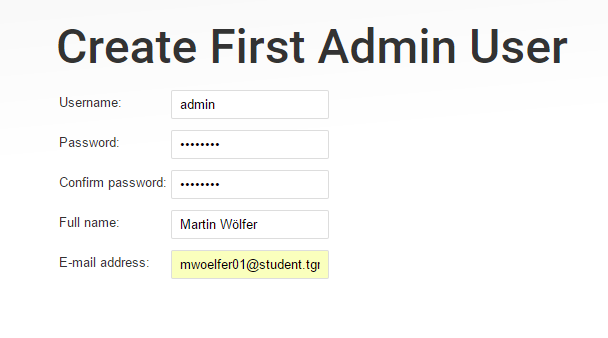
\includegraphics[width=0.8\linewidth]{images/create_admin}
	\figcaption{Ein Admin User wurde erstellt}
\end{minipage}

Anschließend wurde unter \verb|Manage Jenkins|  $\rightarrow$ \verb|Manage plugins| $\rightarrow$ \verb|Available| auch noch das letzte fehlende Plugin installiert (Jenkings Violations).

\subsection{Github-User Konfiguration}
Unter \verb|Manage Jenkins|  $\rightarrow$ \verb|Configure System| $\rightarrow$ \verb|Git Plugin| werden die Daten eingeben. 

\begin{minipage}{\linewidth}
	\centering
	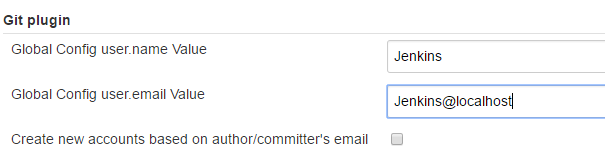
\includegraphics[width=0.8\linewidth]{images/git_plugin}
	\figcaption{Daten werden eingegeben für Git}
\end{minipage}

\section{Ersten Job erstellen}
Im Dashboard wird einem gleich angeboten einen Job zu erstellen, danach wird ein Name für den Job eingeben und es wird \verb|Freestyle Project| ausgewählt

\begin{minipage}{\linewidth}
	\centering
	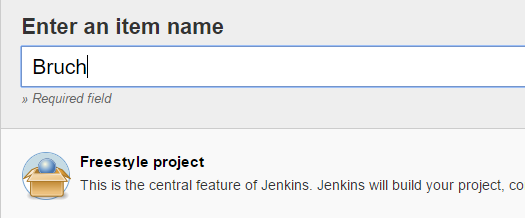
\includegraphics[width=0.8\linewidth]{images/new_job}
	\figcaption{Neuen Job erstellen}
\end{minipage}

\subsection{Job konfigurieren}
\subsubsection{Woher Job Quelle bezieht}
Zuerst muss Jenkins mitgeteilt werden wo die Quelle des Projektes überhaupt liegt, es wird zuerst unter der Section \verb|Source Code Management| der Button \verb|Git| angewählt, und anschließend der lokale Repository URL angegeben werden.

Hier bin ich auf ein weiteres Problem gestoßen, und zwar wurde die Fehlermeldung ausgeben: \textbf{jenkins failed to connect to repository}. Dies lag daran dass Jenkins nicht wusste wo sich lokal mein \verb|git.exe| befindet, daher musste ich in \verb|Manage Jenkins| $\rightarrow$ \verb|Global Tool Configuration| $\rightarrow$ \verb|Git| $\rightarrow$ \verb|Git Installations| den Pfad zu git.exe angeben:

\begin{minipage}{\linewidth}
	\centering
	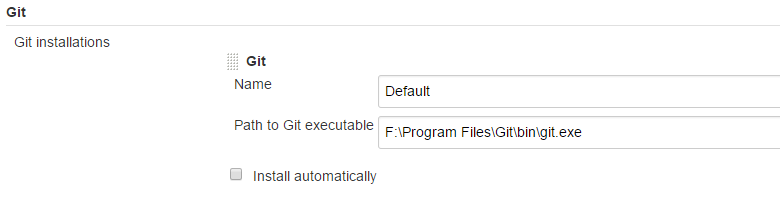
\includegraphics[width=0.6\linewidth]{images/path_to_git}
\end{minipage}

Nun konnte der lokale Pfad zum Repository angegeben werden ohne dass ein Problem besteht:

\begin{minipage}{\linewidth}
	\centering
	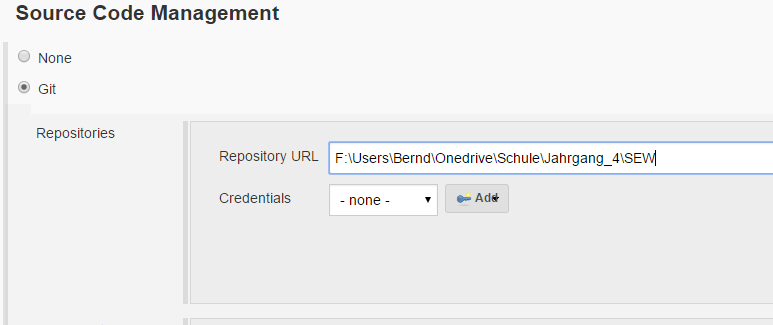
\includegraphics[width=0.8\linewidth]{images/path_to_repo}
	\figcaption{Pfad konnte angegeben werden ohne Fehlermeldung}
\end{minipage}

\subsubsection{Wann Job ausgeführt wird}
Nun wird unter \verb|Build Triggers| $\rightarrow$ \verb|Poll SCM| angegeben wann der Job ausgeführt wird, indem 5 \verb|*| angegeben werden:

\begin{minipage}{\linewidth}
	\centering
	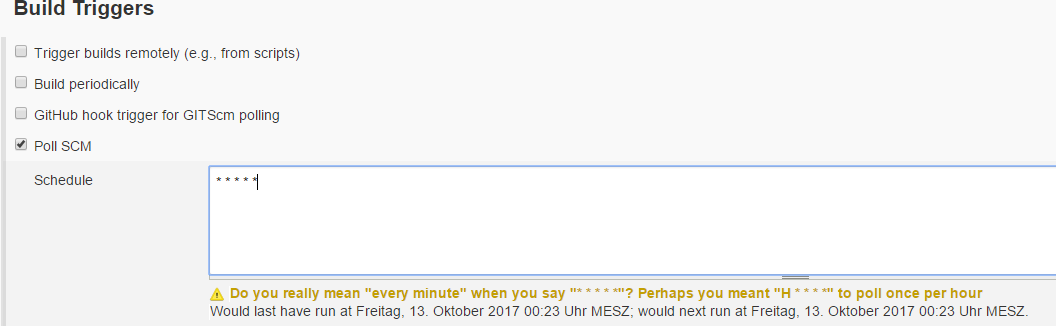
\includegraphics[width=0.8\linewidth]{images/build_triggers}
\end{minipage}

\subsubsection{Was ausgeführt wird}
Unter \verb|Build| $\rightarrow$ \verb|Add build step| $\rightarrow$ \verb|Execute Shell| wird nun folgender Code angegeben:

\begin{lstlisting}[language=bash]
PYTHONPATH=''
nosetests --with-xunit --all-modules --traverse-namespace --with-coverage --cover-package=project1 --cover-inclusive
python -m coverage xml --include=project1*
pylint -f parseable -d I0011,R0801 project1 | tee pylint.out
\end{lstlisting}

\subsubsection{Was passiert mit Ergebnissen}
In diesem Schritt wird nun entschieden wie die Ergebnisse analysiert werden. In diesem Fall werden sie interpretiert durch
\begin{itemize}
	\item Coverage
	\item JUnit testing
	\item Report Violations
\end{itemize}

Unter \verb|Post-build Actions| $\rightarrow$ \verb|Publish Cobertura Coverage Report| wird der Link zum Coverage File angegeben. Es wird lediglich \verb|coverage.xml| angegeben, weil dieses durch den Code im Schritt davor automatisch erzeugt wird.

\begin{minipage}{\linewidth}
	\centering
	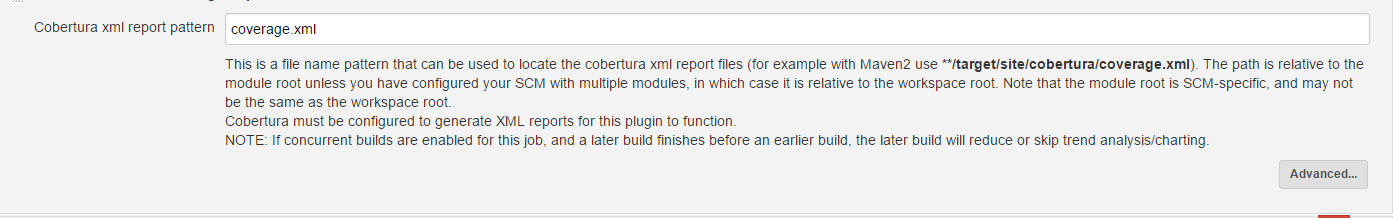
\includegraphics[width=0.8\linewidth]{images/coverage_report}
\end{minipage}

Als nächstes werden die JUnit Test results hinzugefügt. Dazu unter \verb|Post-build Actions| $\rightarrow$ \verb|Publish JUnit test result report| wieder den Filenamen angegeben vom Code erzeugten File, \verb|nosetest.xml|.

\begin{minipage}{\linewidth}
	\centering
	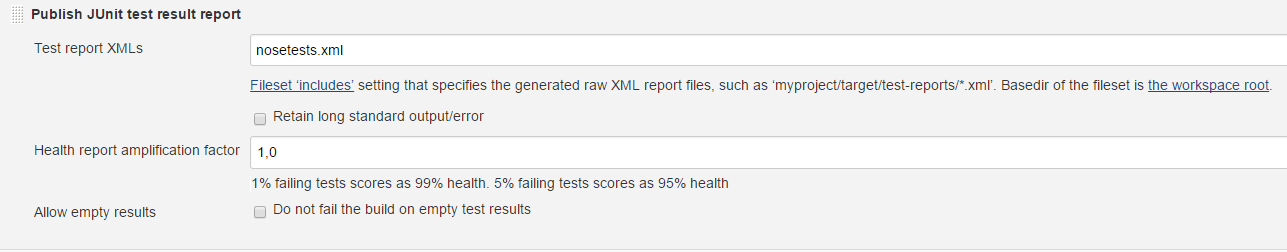
\includegraphics[width=0.8\linewidth]{images/junit_tests}
\end{minipage}

Der letzte Schritt ist es Report Violations zur Interpretation hinzuzufügen. Unter \verb|Post-build Actions| $\rightarrow$ \verb|Report Violations to GitHub| $\rightarrow$ \verb|PYLINT| im Feld \verb|Pattern| folgendes eingeben: \verb|**/pylint.out|. Dieses File wird auch durch den bereits erwähnten Code erstellt.

\begin{minipage}{\linewidth}
	\centering
	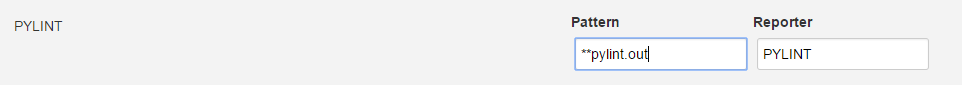
\includegraphics[width=0.8\linewidth]{images/report_violations}
\end{minipage}

Der Job muss nun nur mehr gespeichert werden.

\subsection{Job ausführen}
Dazu wird im Dashboard auf \verb|Build Now| gedrückt. 

\section{Warum es nicht funktioniert}
Wenn der Job gestartet wird, ist der Punkt nicht Grün sondern Rot. Dies indiziert schon mal etwas Schlechtes. Wenn man sich nun den Status ansieht, sieht man nichts. Das bedeutet dass es nicht funktioniert hat weder einen Coverage report, einen JUnit testing report oder einen Report violations report zu erzeugen.

Warum es nicht funktioniert hat, kann man sich im Console Output ansehen:

\begin{lstlisting}[language=bash]
Gestartet durch Benutzer Martin Woelfer
Baue in Arbeitsbereich F:\Program Files (x86)\Jenkins\workspace\Bruch
> F:\Program Files\Git\bin\git.exe rev-parse --is-inside-work-tree # timeout=10
Fetching changes from the remote Git repository
> F:\Program Files\Git\bin\git.exe config remote.origin.url F:\Users\Bernd\Onedrive\Schule\Jahrgang_4\SEW # timeout=10
Fetching upstream changes from F:\Users\Bernd\Onedrive\Schule\Jahrgang_4\SEW
> F:\Program Files\Git\bin\git.exe --version # timeout=10
> F:\Program Files\Git\bin\git.exe fetch --tags --progress F:\Users\Bernd\Onedrive\Schule\Jahrgang_4\SEW +refs/heads/*:refs/remotes/origin/*
> F:\Program Files\Git\bin\git.exe rev-parse "refs/remotes/origin/master^{commit}" # timeout=10
> F:\Program Files\Git\bin\git.exe rev-parse "refs/remotes/origin/origin/master^{commit}" # timeout=10
Checking out Revision efc0ff6d1cb8bc6793162b6a8d8b11047cc90b54 (refs/remotes/origin/master)
> F:\Program Files\Git\bin\git.exe config core.sparsecheckout # timeout=10
> F:\Program Files\Git\bin\git.exe checkout -f efc0ff6d1cb8bc6793162b6a8d8b11047cc90b54
Commit message: "added .pdf"
> F:\Program Files\Git\bin\git.exe rev-list efc0ff6d1cb8bc6793162b6a8d8b11047cc90b54 # timeout=10
[Bruch] $ sh -xe C:\WINDOWS\TEMP\jenkins7976359631185991900.sh
The system cannot find the file specified
FATAL: Befehlsausfuehrung fehlgeschlagen
java.io.IOException: CreateProcess error=2, Das System kann die angegebene Datei nicht finden
at java.lang.ProcessImpl.create(Native Method)
at java.lang.ProcessImpl.<init>(Unknown Source)
at java.lang.ProcessImpl.start(Unknown Source)
Caused: java.io.IOException: Cannot run program "sh" (in directory "F:\Program Files (x86)\Jenkins\workspace\Bruch"): CreateProcess error=2, Das System kann die angegebene Datei nicht finden
at java.lang.ProcessBuilder.start(Unknown Source)
at hudson.Proc$LocalProc.<init>(Proc.java:249)
at hudson.Proc$LocalProc.<init>(Proc.java:218)
at hudson.Launcher$LocalLauncher.launch(Launcher.java:930)
at hudson.Launcher$ProcStarter.start(Launcher.java:450)
at hudson.tasks.CommandInterpreter.perform(CommandInterpreter.java:109)
at hudson.tasks.CommandInterpreter.perform(CommandInterpreter.java:66)
at hudson.tasks.BuildStepMonitor$1.perform(BuildStepMonitor.java:20)
at hudson.model.AbstractBuild$AbstractBuildExecution.perform(AbstractBuild.java:736)
at hudson.model.Build$BuildExecution.build(Build.java:206)
at hudson.model.Build$BuildExecution.doRun(Build.java:163)
at hudson.model.AbstractBuild$AbstractBuildExecution.run(AbstractBuild.java:496)
at hudson.model.Run.execute(Run.java:1724)
at hudson.model.FreeStyleBuild.run(FreeStyleBuild.java:43)
at hudson.model.ResourceController.execute(ResourceController.java:97)
at hudson.model.Executor.run(Executor.java:421)
Build step Shell ausfuehren marked build as failure
[Cobertura] Publishing Cobertura coverage report...
Zeichne Testergebnisse auf.
ERROR: Step Veroeffentliche JUnit-Testergebnisse. failed: Keine JUnit-Testergebnisse gefunden. Liegt vielleicht ein Konfigurationsfehler vor?
---
--- Jenkins Violation Comments to GitHub ---
---
gitHubUrl: 
repositoryOwner: 
repositoryName: 
pullRequestId: 
usernamePasswordCredentialsId: false
username: false
password: false
useOAuth2TokenCredentials: false
oAuth2Token: false
createSingleFileComments: false
createCommentWithAllSingleFileComments: false
commentOnlyChangedContent: false
minSeverity: INFO
keepOldComments: false
PYLINT with pattern **pylint.out
Running Jenkins Violation Comments To GitHub
PR 
Workspace: F:\Program Files (x86)\Jenkins\workspace\Bruch
No pull request id defined, will not send violation comments to GitHub.
Finished: FAILURE
\end{lstlisting}

\subsection{Sh kann nicht ausgeführt werden}
Diese Problem konnte gelöst werden indem in den Settings von Jenkins der Pfad zu \verb|CMD.exe| angegeben wird.

\subsection{Reports werden nicht erzeugt}
Das Problem liegt darin, dass die Befehle welche im Tutorial stehen in meinem System nicht richtig funktionieren. Ich habe probiert wenigstens lokal einen coverage report zu erzeugen, doch bin selbst daran gescheitert da der relative Import mit dem coverage tool nicht funktioniert:


\begin{minipage}{\linewidth}
	\centering
	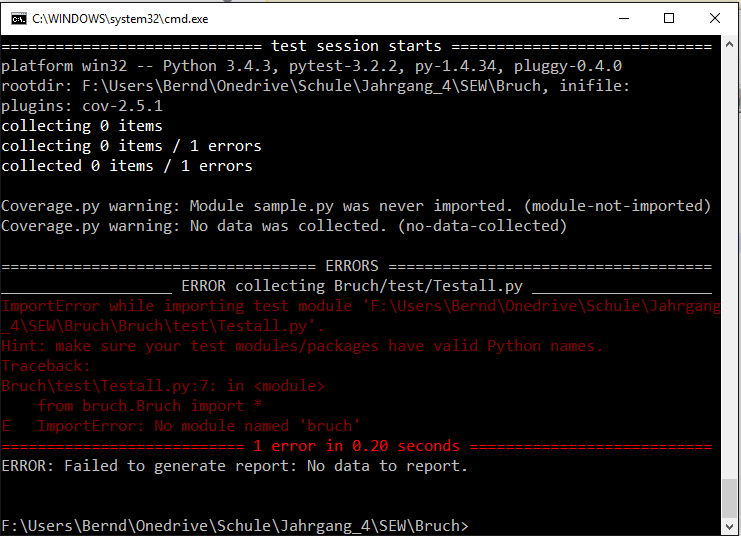
\includegraphics[width=0.8\linewidth]{images/error_python}
\end{minipage}

\subsection{GitHub Link funktioniert nicht}
Es können keine Violation Reports erstellt werden da die Verbindung mit den Github Servern nicht richtig funktioniert.